\section{Introduction}
\label{s:secIntroSM} 
Since ancient times, the human mind has been curious to know more and more
about nature. There have been fundamental questions about the origin of the 
universe and the smallest entity the universe is made of. There have been many 
theoretical and experimental attempts to answer these questions in the past 
centuries. With the advancement in science and technology, we have 
theoretically explained and experimentally verified some of the fundamental building 
blocks of the universe. However, there are still many more questions, for example 
about the origin of dark matter \cite{Ade:2013zuv,Ade:2013sjv}, which we are 
still investigating. None of the 
experiments have directly observed it, although there are many theoretical 
postulates about it. There are many pieces of evidence which suggest that the 
known part of the universe is only about 4\%, rest 96\% are unknown to us. The 
unknown part of the universe is supposed to consist of dark matter and dark energy.

The standard model of particle physics explains the smallest constituents of 
the known part of the matter. As shown in Figure~\ref{fig:scale}, a house 
is made of sand stones, a stone is made of crystals, a crystal is made of atoms, 
an atom is made of nucleons (proton, neutron) and electrons, a proton (or neutron) 
is made of quarks. The quark and electron are the fundamental particles, that is, 
they are not made of any other sub-particles. Therefore, the whole known universe
is made of these fundamental particles by combining them in appropriate proportions.
There are other fundamental particles which mediate the force which binds the 
quarks to form a proton or neutron.
\begin{figure}
  \begin{center}
  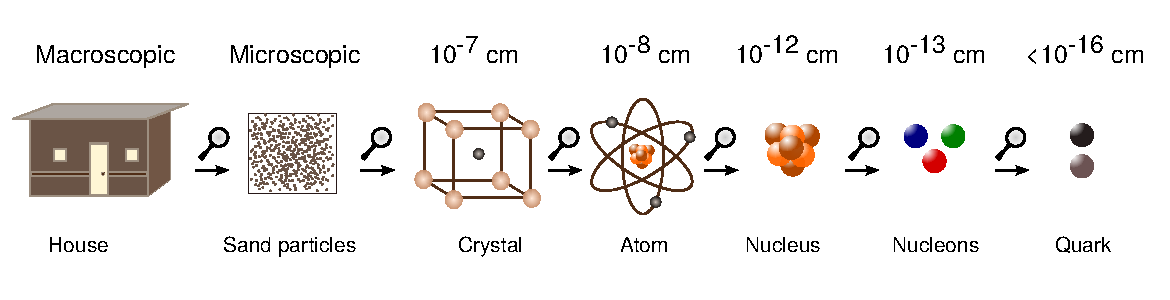
\includegraphics[width=1.0\linewidth]{Theory/Image/scale.pdf}
	  \caption{A schematic picture showing the hierarchy of building blocks
	  of the matter when one looks deeper and deeper, from right to left.
	  This figure is adopted from \cite{scienceabc}.}
  \label{fig:scale}
  \end{center}
\end{figure}

The quarks are of different types such as \textit{up} quark (\PQu), \textit{down} quark (\PQd), 
\textit{charm} quark (\PQc), \textit{strange} quark (\PQs), \textit{top} quark (t), and \textit{bottom}
quark (\PQb). The mass of each quark is different. The electric charge is 2/3 for \PQu, \PQc, \PQt 
quarks and -1/3 for \PQs, \PQb, and \PQd quarks. The electron has different partners such as 
\textit{muon} ($\mu$) and \textit{tau} ($\tau$). They differ in mass only, the electric charge 
is the same. The electron, muon, and tau are collectively called leptons. There are also 
electric-neutral partners of leptons called neutrinos such as \textit{electron-neutrino} ($\nu_e$), 
\textit{muon-neutrino} ($\nu_\mu$), and \textit{tau-neutrino} ($\nu_\tau$). The quarks are bound 
by a strong force mediated by a \textit{gluon}. The leptons interact themselves by an electromagnetic 
force mediated by a \textit{photon}. The lepton and neutrino interact by electro-weak force 
mediated by the \PW and \PZ boson. The quarks, leptons, photon, gluon, \PW/\PZ boson are 
the fundamental particles. The mass to these particles is given
by another fundamental particle called the \textit{Higgs} boson. The mass, electric charge,
and spin of all the fundamental particles are shown in Figure~\ref{fig:sm_particles}.
\begin{figure}
  \begin{center}
  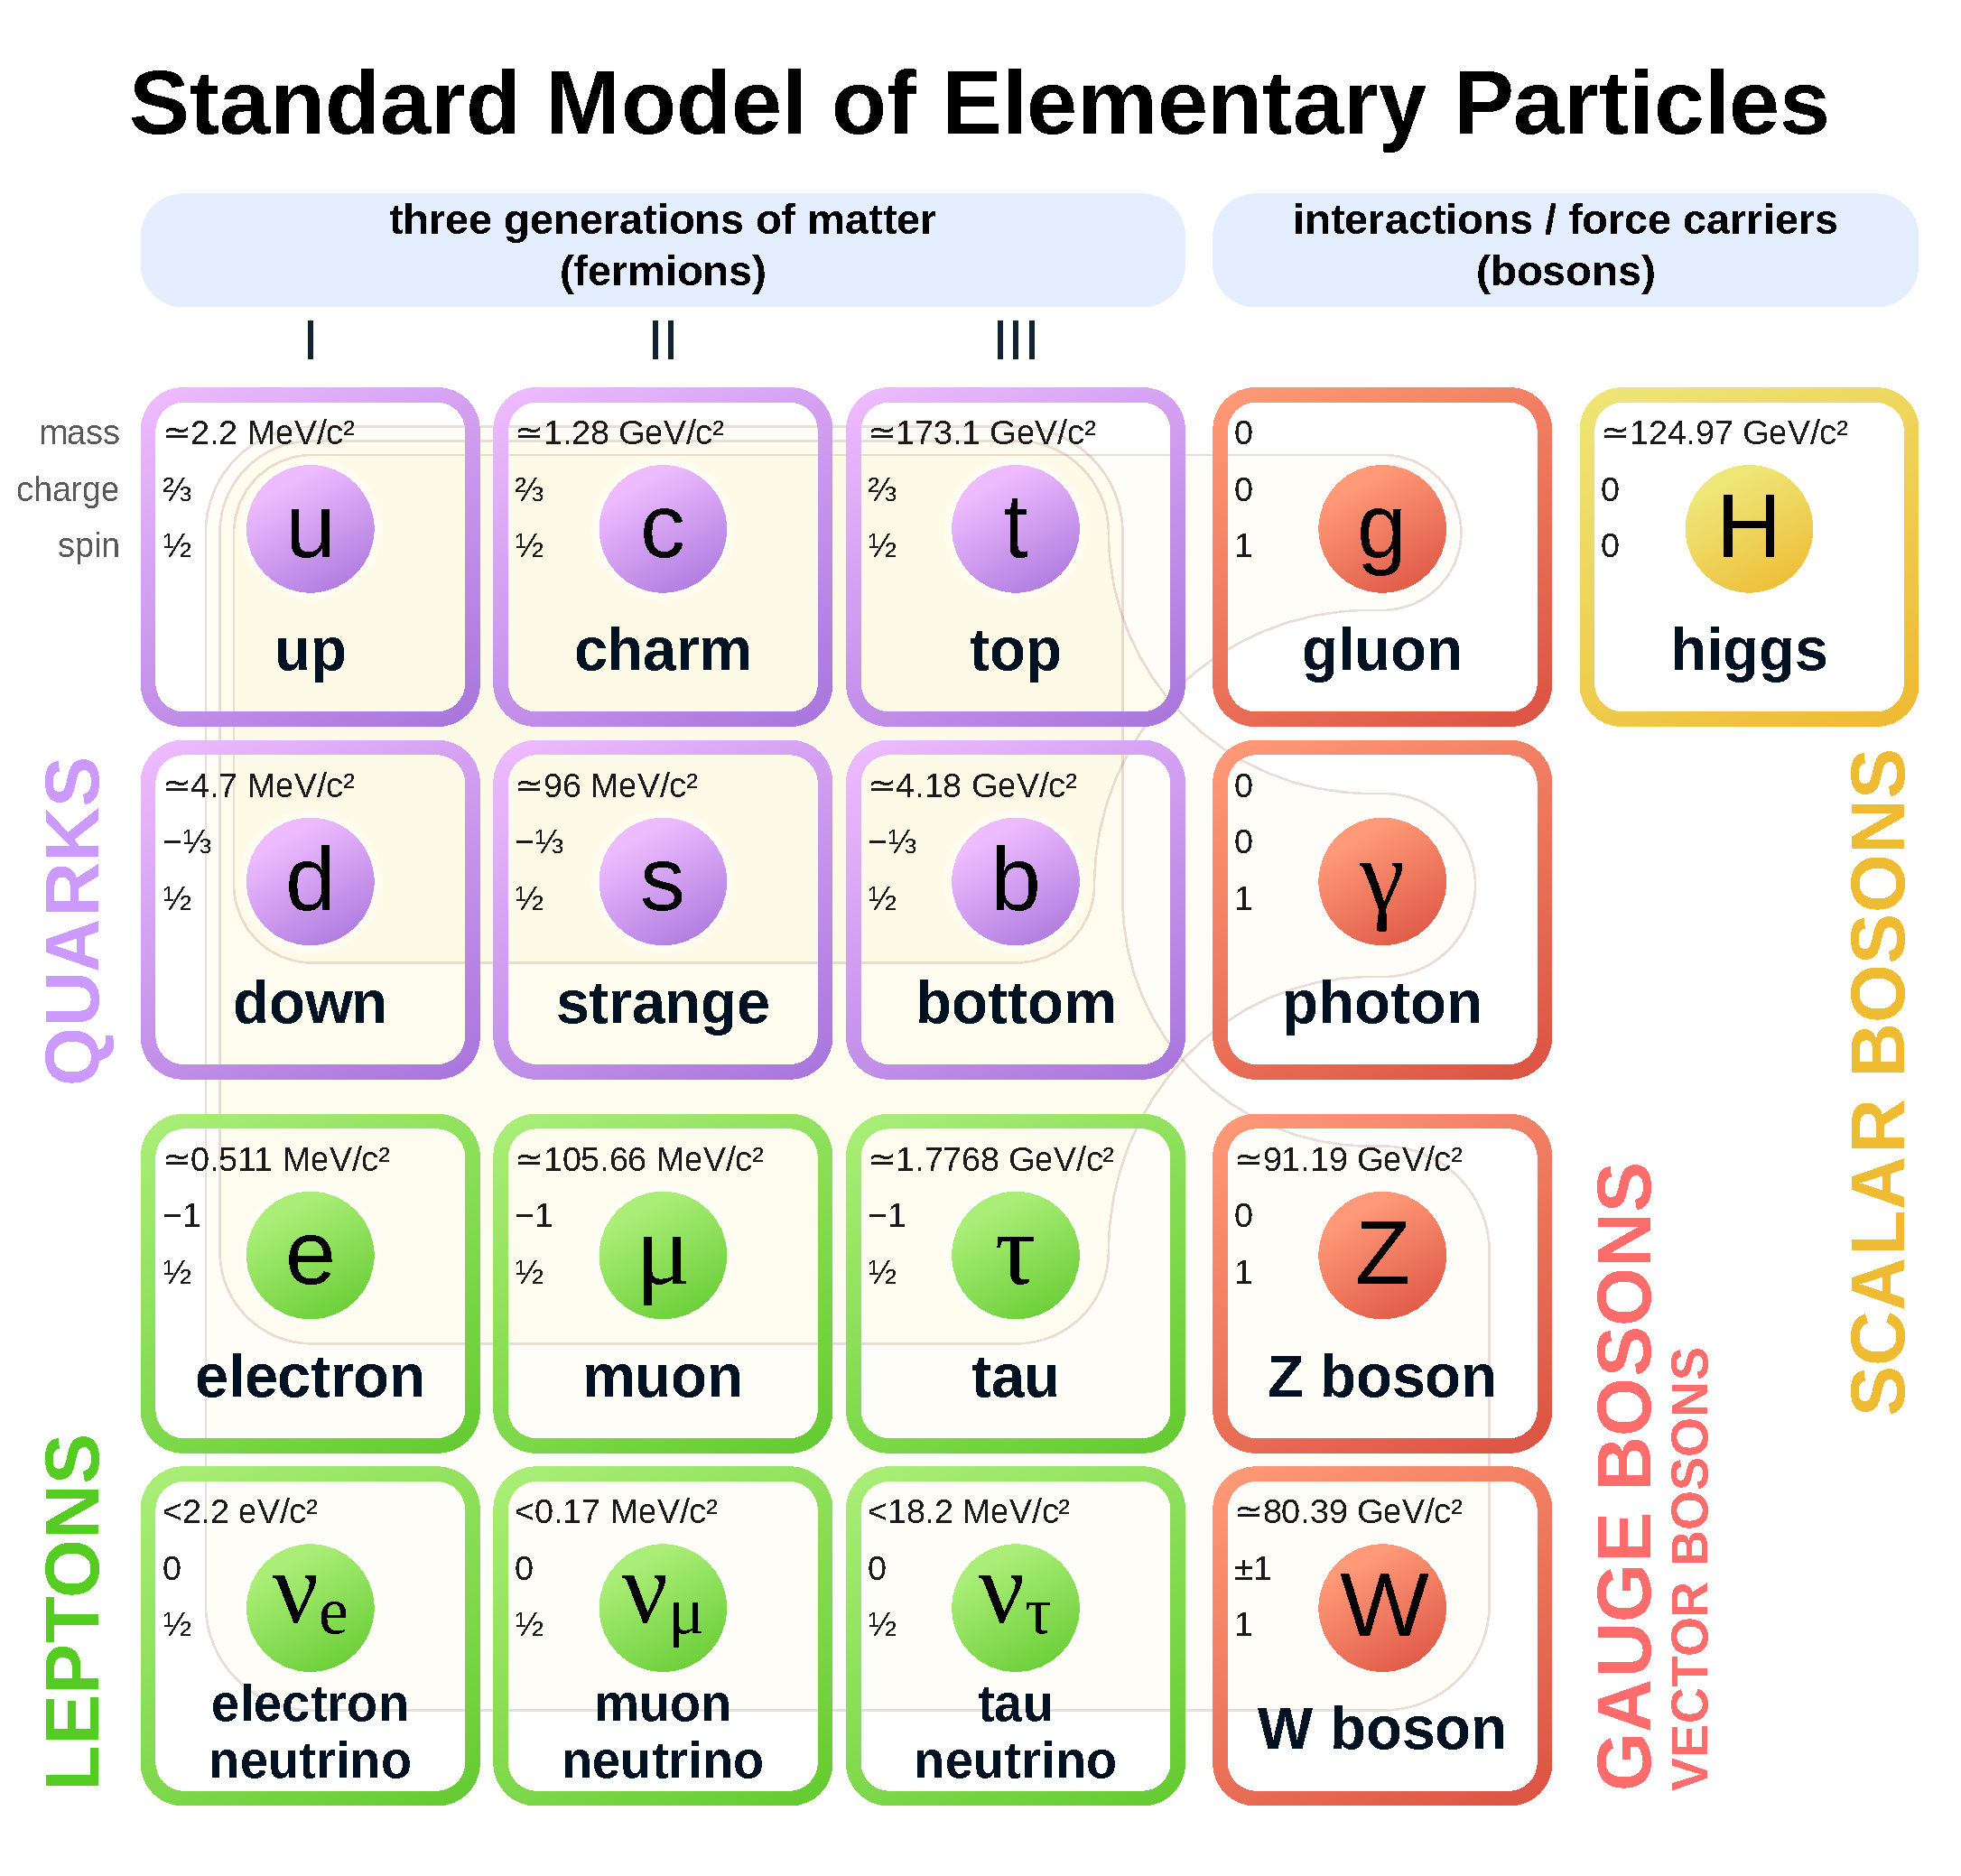
\includegraphics[width=0.80\linewidth]{Theory/Image/sm_particles.pdf}
\caption{Physical properties of the fundamental particles\cite{wikiSM}. 
	There are three generations of quarks and leptons grouped in the increasing
	order of mass. The gluon, photon, Z/W, and Higgs  bosons are force carriers.} 
  \label{fig:sm_particles}
  \end{center}
\end{figure}
All the composite particles are made of fundamental particles. All the physics
process in nature involves interactions between the fundamental particles. 
The standard model of particle physics describe all the interactions of the fundamental particles, 
as shown in Figure~\ref{fig:particle_int}. Here the photon can interact with a lepton, 
quarks, and W boson. The gluon can interact with only quarks and itself. The Higgs
boson interacts with itself, electron, muon, tau, \PW, \PZ, and all the quarks. 

The discovery of all the fundamental particles took centuries. Some of them were 
theoretically predicted many years before being experimentally observed.
The timeline of the fundamental particles are shown in Figure~\ref{fig:particle_timeline}. 
The electron was the first elementary particle to
be theorized and discovered in the late 19$^{\rm{th}}$ century. The photon, electron-neutrino,
and muon were discovered in the first 50\unit{yrs} of the 20$^{\rm{th}}$ century. All the quarks, 
except the \PQt quark, were discovered in the 60's and 70's of the 20$^{\rm{th}}$ century. The
Higgs boson is the only particle discovered in the 21$^{\rm{st}}$ century which took 48\unit{yrs}, 
it was theoretically predicted in 1964. A brief history of elementary particles 
can be found in \cite{Griffiths:111880}.
\begin{figure}
  \begin{center}
  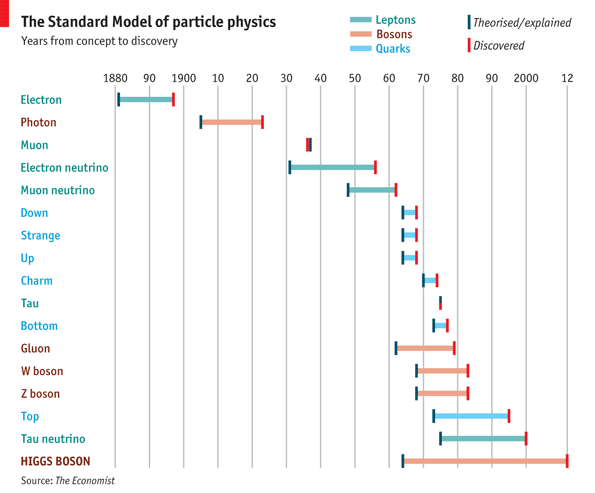
\includegraphics[width=0.75\linewidth]{Theory/Image/particle_timeline.png}
	  \caption{A timeline of the fundamental particles from their theoretical 
	prediction to the experimental observation.}
  \label{fig:particle_timeline}
  \end{center}
\end{figure}

\begin{figure}
  \begin{center}
  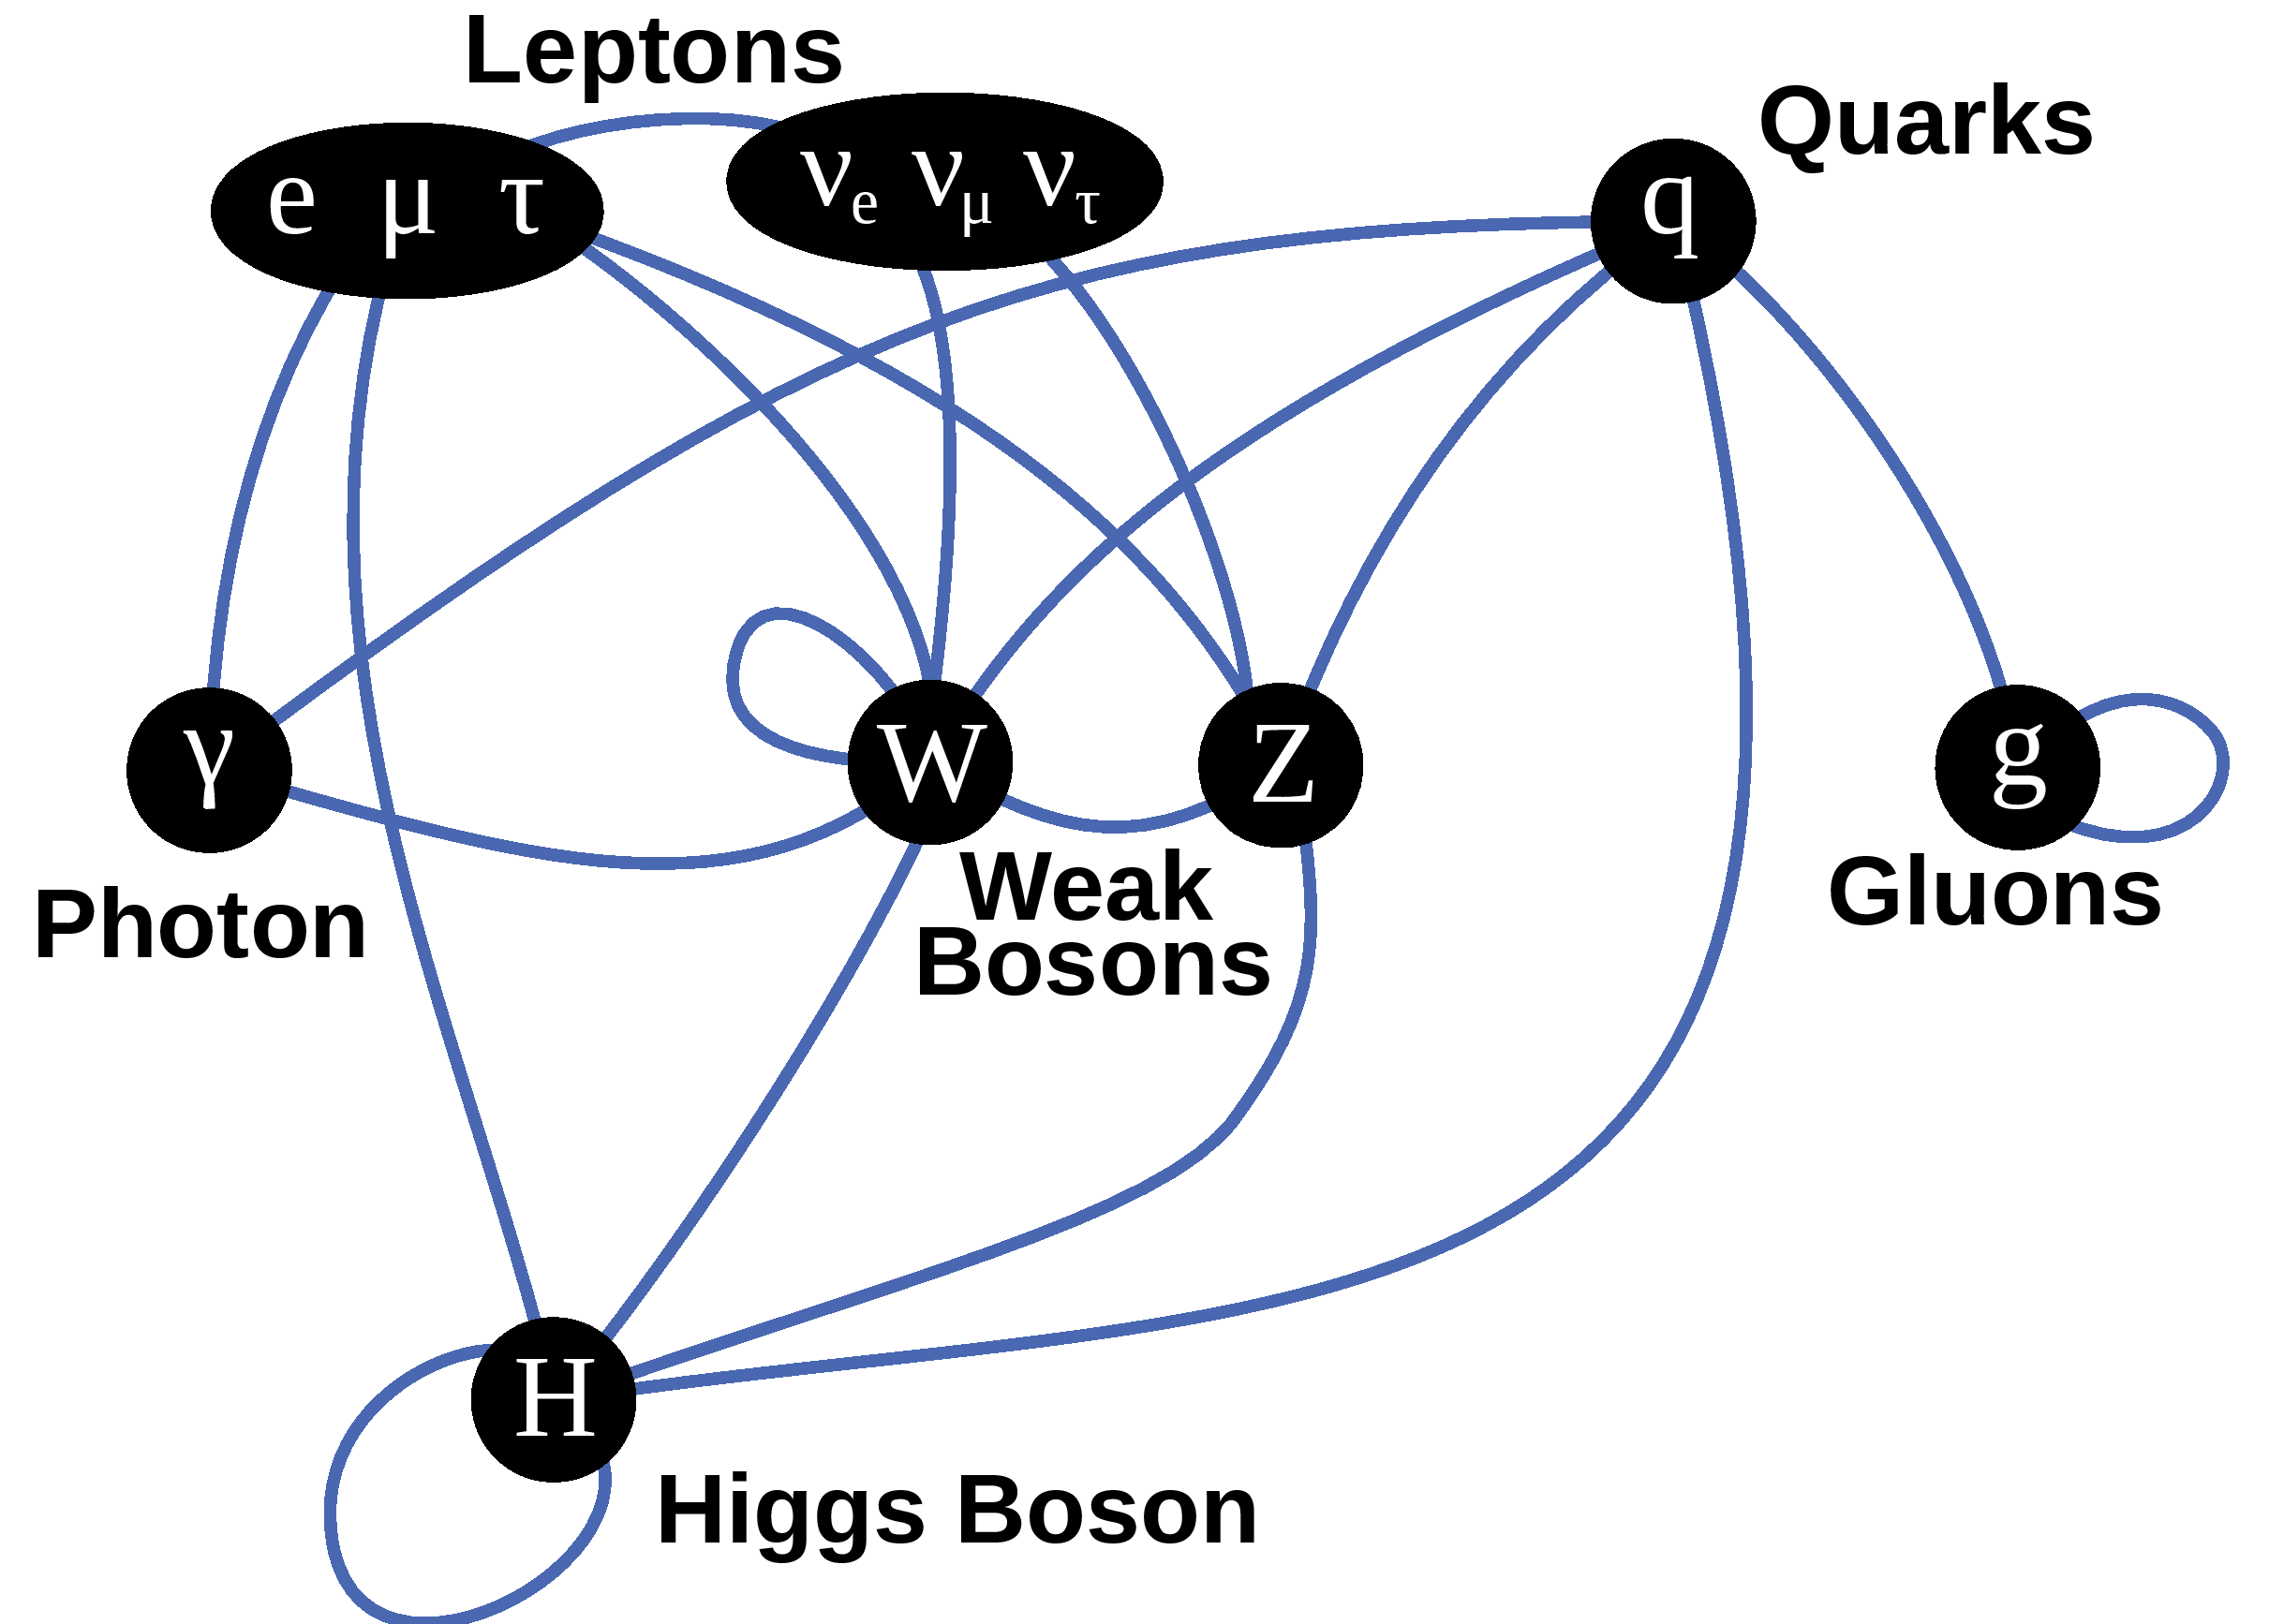
\includegraphics[width=0.50\linewidth]{Theory/Image/particle_int.png}
	\caption{A schematic diagram showing the interactions of fundamental 
	particles among themselves\cite{Isildak:2013kfa}.} 
  \label{fig:particle_int}
  \end{center}
\end{figure}

